%%----------------------------------------------------------------------------------------
\clearpage
\pagestyle{fancy}
%%----------------------------------------------------------------------------------------
%%       PREFAZIONE
%%----------------------------------------------------------------------------------------
\part{Risoluzione delle strutture staticamente determinate}
\setcounter{section}{0}
\section{Introduzione}
%----------------------------------------------------------------------------------------
Una volta che la struttura è stata classificata, se essa è \textsc{in equilibrio} ed è \textsc{staticamente determinata}, cioè se $i=0$, lo strutturista è chiamato a calcolarne le \textsc{reazioni vincolari}. Si tratta, ovviamente, \textbf{di scrivere le equazioni di equilibrio e}, \textbf{poi}, \textbf{di risolvere il sistema}~\eqref{equazione7-1}; e ciò, naturalmente, non costituisce alcun problema se si vuole la risoluzione numerica: basta usare un computer. Tuttavia, specie in sede di progettazione preliminare, è utile pervenire alla risoluzione letterale del sistema, essendovi dei coefficienti ancora non definiti in termini numerici. In questa \emph{ottica} sarà bene ricorrere ad una adeguata metodologia che consenta di \textbf{accorciare i tempi}. L'idea di base è la seguente: 
%----------------------------------------------------------------------------------------
%--------------------------------------------------------------------------------------------------------------------------------------------------------------
\\

\fbox{\begin{minipage}{38em}
\centering
\textsc{È decisamente preferibile frazionare il sistema~\eqref{equazione7-1} in più sottosistemi di dimensione minore.}
\end{minipage}}
\\
\\

%--------------------------------------------------------------------------------------------------------------------------------------------------------------
%----------------------------------------------------------------------------------------
\noindent Tanto per intenderci, è di gran lunga preferibile risolvere una serie di sistemi $3\times 3$ o $2\times 2$ piuttosto che un solo sistema $8\times 8$. 
%----------------------------------------------------------------------------------------
\section{Alcuni notevoli casi di equilibrio}
%----------------------------------------------------------------------------------------
Nelle strutture bidimensionali, come è noto, le forze attive e reattive sono complanari (agiscono nello stesso piano). Le condizioni di equilibrio più comuni nel caso di forze complanari possono essere formulate in termini geometrici. Eccole:
%----------------------------------------------------------------------------------------
\begin{itemize}
\item \textsc{Due forze sono in equilibrio \textbf{se e solo se} formano una coppia di braccio nullo.}
\item \textsc{Due (o più) forze più un momento sono in equilibrio \textbf{se e solo se} le due (o più) forze formano una coppia il cui momento è uguale ed opposto a quello assegnato.}
\item \textsc{Condizione necessaria affinché tre forze siano in equilibrio è che esse concorrano in un punto oppure che esse siano parallele.}
\end{itemize}
%----------------------------------------------------------------------------------------
\section{Una metodologia per la risoluzione delle strutture a più tronchi}
%----------------------------------------------------------------------------------------
Premettiamo alcune definizioni:
%----------------------------------------------------------------------------------------
%----------------------------------------------------------------------------------------
\renewcommand{\thefigure}{8~-~1}
\begin{figure}[ht]
\centering
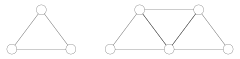
\includegraphics[width=0.65\textwidth]{Immagini/Parte_8/Figura8_1/Figura8_1.pdf}
\caption{}
\label{figura8-1}
\end{figure}
%---------------------------------------------------------------------------------------
\begin{description}
%----------------------------------------------------------------------------------------
\item[Struttura isostatica per vincoli esterni:] Viene così definita ogni struttura i cui vincoli esterni comportino $3$ \textsc{incognite}. È ovvio che, scrivendo le $3$ \textsc{equazioni di equilibrio esterno}, si otterrà un sistema $3\times 3$ e si potranno calcolare agevolmente le $3$ \textsc{reazioni esterne}. Naturalmente, se il carico attivo è \textsc{autoequilibrato} e cioè si ha
%----------------------------------------------------------------------------------------
\begin{align*}
\underline{R}^{(a)} &= \underline{0} \\
\underline{M}^{(a)} &= \underline{0}
\end{align*}
%----------------------------------------------------------------------------------------
il suddetto sistema sarà omogeneo e le reazioni esterne saranno tutte nulle;
%----------------------------------------------------------------------------------------
\item[Tronco isostatico:] Viene così definito un tronco tale che i vincoli afferenti ad esso comportino $3$ \textsc{incognite}. È ovvio che, scrivendo le $3$ \textsc{equazioni di equilibrio del tronco}, si otterrà un sistema $3\times 3$ e si potranno determinare le $3$ \textsc{incognite}. Naturalmente se il tronco è scarico oppure il carico agente su di esso è autoequilibrato, il suddetto sistema sarà omogeneo e le reazioni dei vincoli afferenti al tronco saranno tutte nulle;
%----------------------------------------------------------------------------------------
\item[Blocco rigido isostatico per vincoli di frontiera:] Un insieme di tronchi e/o punti materiali vincolati tra loro in maniera tale che non vi possano essere spostamenti relativi si dice che costituisce un \textsc{blocco rigido}. Un esempio molto frequente di blocco rigido è una \textsc{maglia triangolare} o una \textsc{serie di più maglie triangolari}, aventi un lato in comune l'una con l'altra (si osservi la figura~\ref{figura8-1}). Una maglia triangolare è, in effetti, un complesso di $3$ tronchi i cui centri relativi \textsc{non sono allineati} e perciò essa forma un blocco rigido. I vincoli di frontiera di un blocco rigido sono, naturalmente quelli che lo collegano al suolo o alle altre parti costituenti la struttura. Un blocco si dice \textsc{isostatico per vincoli di frontiera} se questi comportano $3$ incognite. Ciò detto, un blocco rigido può assimilarsi ad un tronco e vale quanto detto per il tronco isostatico. 
%----------------------------------------------------------------------------------------
\item[Tronco $1$ volta iperstatico:] Viene così definito un tronco tale che i vincoli afferenti ad esso comportino $4$ incognite;
%----------------------------------------------------------------------------------------
\item[Nodo~-~cerniera staticamente determinato:] Viene così definito un nodo~-~cerniera tale che i vincoli afferenti ad esso comportino $2$ incognite.
%----------------------------------------------------------------------------------------
\end{description}
%----------------------------------------------------------------------------------------
\noindent Ciò premesso, ecco come conviene procedere allorché si vuole risolvere una struttura:
%----------------------------------------------------------------------------------------
\begin{enumerate}
%----------------------------------------------------------------------------------------
\item Se la struttura è \textsc{isostatica per vincoli esterni} si cominciano a scrivere le $3$ equazioni di equilibrio esterno e si trovano agevolmente le reazioni di questi ultimi. Successivamente si scriveranno le equazioni di equilibrio di un tronco che sia divenuto isostatico e così via; se la struttura non è isostatica per vincoli esterni allora si faccia riferimento al punto seguente.
%----------------------------------------------------------------------------------------
\item Se la struttura presenta un \textsc{tronco isostatico}, se ne cominciano a scrivere le equazioni di equilibrio e si trovano agevolmente le tre equazioni dei vincoli afferenti ad esso. Dopo di che si passa ad un altro equilibrio, per esempio quello esterno, se ora le incognite di terra sono diventate $3$, oppure quelle di un altro tronco isostatico. Se quanto detto sino ad ora risulta impraticabile, si faccia riferimento ai punti seguenti.
%----------------------------------------------------------------------------------------
\item Se la struttura presenta un \textsc{blocco rigido isostatico} per vincoli di frontiera si assimila il blocco rigido ad un tronco e si procede così come illustrato al punto due. 
%----------------------------------------------------------------------------------------
\item Se la struttura presenta un \textsc{nodo~-~cerniera staticamente determinato} se ne cominciano a scrivere le equazioni di equilibrio e si trovano agevolmente le $2$ reazioni dei vincoli afferenti in esso. 
%----------------------------------------------------------------------------------------
\item Se la struttura presenta un \textsc{tronco $1$ volta iperstatico} non soggetto a forze attive, o soggetto a forze attive \emph{particolari}, si comincia a \emph{ragionare} sul suo equilibrio: in tal modo, pur essendo impossibile determinare le reazioni su di esso poiché si avrebbe un sistema di $3$ equazioni in $4$ incognite, si acquisirà un \emph{nuovo indizio} che aprirà \emph{nuove strade}. 
%----------------------------------------------------------------------------------------
\item Se la struttura presenta un \textsc{blocco rigido $1$ volta iperstatico} per vincoli di frontiera si procede come descritto al punto precedente.
%----------------------------------------------------------------------------------------
\item Se la struttura è \textsc{$1$ volta iperstatica per vincoli esterni} ed il \textbf{carico attivo è autoequlibrato}, allora saranno autoequilibrate anche le reazoni di terra; questo \emph{nuovo indizio} aprirà dunque \emph{nuove strade}.
%----------------------------------------------------------------------------------------
\end{enumerate}
%----------------------------------------------------------------------------------------
\noindent Concludiamo il paragrafo con una importante precisazione: è emerso che, oltre alle $m$ equazioni di equilibrio delle parti costituenti, $3$ per ogni tronco più $2$ per ogni punto materiale, sono anche disponibili le $3$ equazioni di equilibrio esterno. Così, si potrebbe pensare che le equazioni di equilibrio per una struttura a più tronchi siano in realtà $m+3$. La verità, però, è che di queste $m+3$ equazioni di equilibrio solo $m$ sono \textsc{linearmente indipendenti}; le ulteriori $3$ equazioni possono essere utilizzate come un \emph{valido strumento di verifica}.
%--------------------------------------------------------------------------------------------------------------------------------------------------------------
\clearpage
\section{Esercizi}
\paragraph{Esercizio 8.1}
La struttura rappresentata in figura~\ref{Esercizio8-1-1} e, con essa, tutte le strutture costituite da $2$ o più tronchi rettilinei allineati, prende il nome di \textsc{trave Gerber}. Ciò premesso, si chiede:
%--------------------------------------------------------------------------------------------------------------------------------------------------------------
\begin{enumerate}
\item di classificarla;
\item di determinare, se possibile, le reazioni vincolari.
\end{enumerate}
%--------------------------------------------------------------------------------------------------------------------------------------------------------------
\renewcommand{\thefigure}{8.1~-~1}
\begin{figure}[ht]
\centering
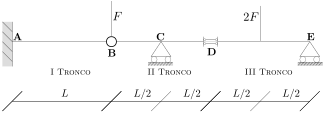
\includegraphics[width=\textwidth]{Immagini/Parte_8/Esercizio8_1/Esercizio8_1_1.pdf}
\caption{}
\label{Esercizio8-1-1}
\end{figure}
%--------------------------------------------------------------------------------------------------------------------------------------------------------------
\subparagraph{Quesito 1:}
\noindent Chiaramente, la struttura è divisa nei $3$ \textsc{tronchi} $\mathbf{A}\mathbf{B}$, $\mathbf{B}\mathbf{D}$ e $\mathbf{D}\mathbf{E}$. Dunque
%----------------------------------------------------------------------------------------
\begin{align*}
m &= 3\times 3 = 9 \\
n &= 3\mathbf{A}+2\mathbf{B}+1\mathbf{C}+2\mathbf{D}+1\mathbf{E} = 9
\end{align*}
%----------------------------------------------------------------------------------------
\noindent da cui è ovvio scrivere la seguente
%----------------------------------------------------------------------------------------
\begin{equation*}
m-n = l-i = 0
\end{equation*}
%----------------------------------------------------------------------------------------
Osservando la trave nell'ottica della cinematica, appare evidente che nessun tronco può muoversi; dunque $l=0$. Conseguentemente anche $i=0$. La struttura è dunque \textsc{isostatica}. Essa è pertanto \textsc{in equilibrio per ogni carico attivo} e le reazioni vincolari sono \textsc{univocamente determinate}. 
%----------------------------------------------------------------------------------------
\noindent \subparagraph{Quesito 2:}
Anziché scrivere il sistema $9\times 9$, cercheremo di frazionarlo in sottosistemi $3\times 3$ utilizzando le tecniche esposte nei paragrafi precedenti. Il \textsc{III Tronco} è isostatico e perciò inizieremo ad imporre il suo equilibrio.
%--------------------------------------------------------------------------------------------------------------------------------------------------------------
\renewcommand{\thefigure}{8.1~-~2}
\begin{figure}[ht]
\centering
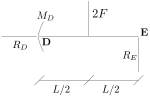
\includegraphics[width=0.525\textwidth]{Immagini/Parte_8/Esercizio8_1/Esercizio8_1_4.pdf}
\caption{}
\label{Esercizio8-1-2}
\end{figure}
%--------------------------------------------------------------------------------------------------------------------------------------------------------------
Facendo riferimento alla figura~\ref{Esercizio8-1-2}, si ha
%--------------------------------------------------------------------------------------------------------------------------------------------------------------
\begin{align*}
R_D &= 0 \quad [\to] \\ 
R_E - 2F &= 0 \quad [\uparrow] \\
-M_D + 2F\frac{L}{2} &=0 \quad [\mathbf{E}\circlearrowleft]
\end{align*}
%----------------------------------------------------------------------------------------
Quindi si ricava immediatamente
%--------------------------------------------------------------------------------------------------------------------------------------------------------------
\begin{align*}
R_D &= 0 \quad [\to] \\ 
R_E &= 2F \quad [\uparrow] \\
M_D &= FL \quad [\mathbf{E}\circlearrowright]
\end{align*}
%----------------------------------------------------------------------------------------
Con il simbolo $\mathbf{E}\circlearrowright$ si indica il polo di calcolo del momento ed il verso adottato come positivo nel calcolo. Si noti che il momento $M_D$ ipotizzato orario si è rivelato essere in realtà antiorario. Noti $R_D$ ed $M_D$, ora il \textsc{III Tronco} è diventato isostatico; su di esso, contiamo tre incognite $H_B$, $V_B$ ed $R_C$ e pertanto andremo ad imporre il suo equilibrio.
%--------------------------------------------------------------------------------------------------------------------------------------------------------------
\renewcommand{\thefigure}{8.1~-~3}
\begin{figure}[ht]
\centering
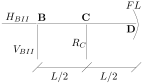
\includegraphics[width=0.525\textwidth]{Immagini/Parte_8/Esercizio8_1/Esercizio8_1_5.pdf}
\caption{}
\label{Esercizio8-1-3}
\end{figure}
%--------------------------------------------------------------------------------------------------------------------------------------------------------------
Facendo riferimento alla figura~\ref{Esercizio8-1-3} si ha
%--------------------------------------------------------------------------------------------------------------------------------------------------------------
\begin{align*}
H_{BII} &= 0 \quad [\to] \\ 
V_{BII} + R_C &= 0 \quad [\uparrow] \\
R_{C}\frac{L}{2} + FL &=0 \quad [\mathbf{B}\circlearrowleft]
\end{align*}
%----------------------------------------------------------------------------------------
e si ricava immediatamente che
%--------------------------------------------------------------------------------------------------------------------------------------------------------------
\begin{align*}
H_{BII} &= 0 \quad [\to] \\ 
V_{BII} &= 2F \quad [\uparrow] \\
R_{C} &=-2F \quad [\downarrow]
\end{align*}
%----------------------------------------------------------------------------------------
%--------------------------------------------------------------------------------------------------------------------------------------------------------------
\renewcommand{\thefigure}{8.1~-~4}
\begin{figure}[ht]
\centering
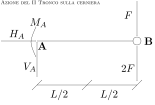
\includegraphics[width=0.525\textwidth]{Immagini/Parte_8/Esercizio8_1/Esercizio8_1_6.pdf}
\caption{}
\label{Esercizio8-1-4}
\end{figure}
%--------------------------------------------------------------------------------------------------------------------------------------------------------------
Passiamo infine al \textsc{I Tronco}, che ora è diventato isostatico; si ha
%----------------------------------------------------------------------------------------
\begin{align*}
H_{A} &= 0 \quad [\to] \\ 
V_{A} &= 3F \quad [\uparrow] \\
M_{A} &=-3FL \quad [\mathbf{A}\circlearrowleft]
\end{align*}
%----------------------------------------------------------------------------------------
Si ricava immediatamente  quanto segue
%----------------------------------------------------------------------------------------
\begin{align*}
H_{A} &= 0 \quad [\to] \\ 
V_{A} &= 3F \quad [\uparrow] \\
M_{A} &=3FL \quad [\mathbf{A}\circlearrowright]
\end{align*}
%----------------------------------------------------------------------------------------
%--------------------------------------------------------------------------------------------------------------------------------------------------------------
\renewcommand{\thefigure}{8.1~-~5}
\begin{figure}[ht]
\centering
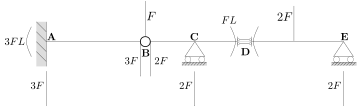
\includegraphics[width=\textwidth]{Immagini/Parte_8/Esercizio8_1/Esercizio8_1_2.pdf}
\caption{}
\label{Esercizio8-1-5}
\end{figure}
%--------------------------------------------------------------------------------------------------------------------------------------------------------------
Ed ecco il quadro completo delle reazioni, rappresentato in figura~\ref{Esercizio8-1-5}. 
%--------------------------------------------------------------------------------------------------------------------------------------------------------------
\renewcommand{\thefigure}{8.1~-~6}
\begin{figure}[ht]
\centering
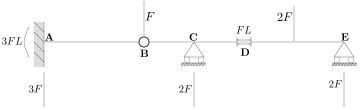
\includegraphics[width=\textwidth]{Immagini/Parte_8/Esercizio8_1/Esercizio8_1_3.pdf}
\caption{}
\label{Esercizio8-1-6}
\end{figure}
%--------------------------------------------------------------------------------------------------------------------------------------------------------------
L'equilibrio esterno non è stato fin qui utilizzato; potremmo utilizzarlo per verificare l'esattezza dei risultati, partendo dalla figura~\ref{Esercizio8-1-6}
%----------------------------------------------------------------------------------------
\begin{align*}
0 &= 0 \quad [\to] \quad \boxed{\textup{Ok!}} \\ 
3F-F-2F-2F+2F &= 0 \quad [\uparrow]  \quad \boxed{\textup{Ok!}} \\
3FL-FL-2F\frac{3}{2}L-2F\frac{5}{2}L+2F\cdot 3L &=0 \quad [\circlearrowright] \quad \boxed{\textup{Ok!}}
\end{align*}
%----------------------------------------------------------------------------------------
%--------------------------------------------------------------------------------------------------------------------------------------------------------------
\clearpage
\paragraph{Esercizio 8.2}
Si chiede di
\begin{itemize}
\item classificare la struttura rappresentata in figura~\ref{Esercizio8-2-1}; 
\item determinare, se possibile, le reazioni vincolari.
\end{itemize}
%--------------------------------------------------------------------------------------------------------------------------------------------------------------
%--------------------------------------------------------------------------------------------------------------------------------------------------------------
\renewcommand{\thefigure}{8.2~-~1}
\begin{figure}[ht]
\centering
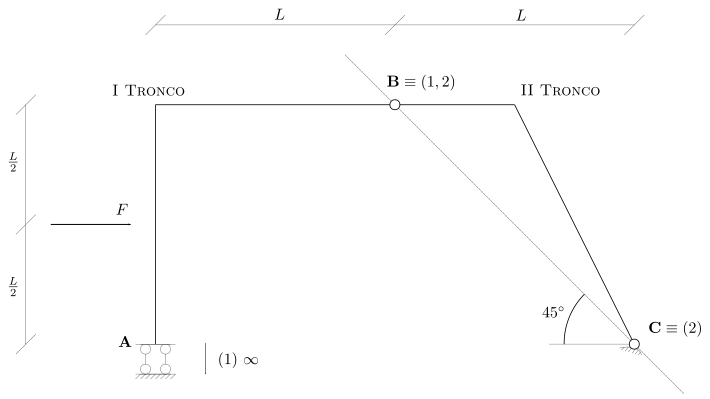
\includegraphics[width=\textwidth]{Immagini/Parte_8/Esercizio8_2/Esercizio8_2_1.pdf}
\caption{}
\label{Esercizio8-2-1}
\end{figure}
%--------------------------------------------------------------------------------------------------------------------------------------------------------------
\noindent \subparagraph{Quesito 1:}
%----------------------------------------------------------------------------------------
Si ha 
%----------------------------------------------------------------------------------------
\begin{align*}
m    &= 2\times 3 = 6 \\ 
n     &= 2\mathbf{A}+2\mathbf{B}+2\mathbf{C} = 6 \\
m-n &= l-i = 0  
\end{align*}
%----------------------------------------------------------------------------------------
I centri assoluti ed il centro relativo sono univocamente determinati ma \textsc{non allineati}: ciò vuol dire che $l=0$; conseguentemente $i=0$ e quindi la struttura è \textsc{isostatica}. 
%----------------------------------------------------------------------------------------
\noindent \subparagraph{Quesito 2:}
%--------------------------------------------------------------------------------------------------------------------------------------------------------------
\renewcommand{\thefigure}{8.2~-~2}
\begin{figure}[ht]
\centering
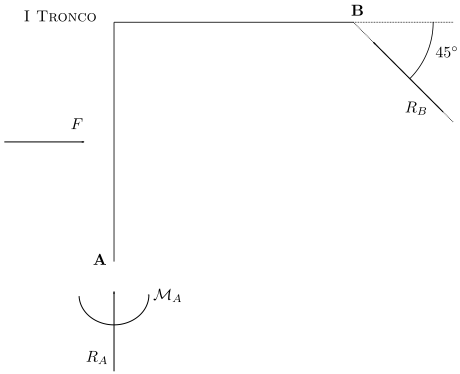
\includegraphics[width=0.55\textwidth]{Immagini/Parte_8/Esercizio8_2/Esercizio8_2_2.pdf}
\caption{}
\label{Esercizio8-2-2}
\end{figure}
%--------------------------------------------------------------------------------------------------------------------------------------------------------------
Cominciamo a ragionare sull'equilibrio del \textsc{II Tronco}, che è $1$ \textsc{volta iperstatico} e non è soggetto a forze attive: su di esso agiscono due forze $\underline{R}_C$ ed $\underline{R}_{IIB}$; esse devono formare una coppia di braccio nullo e, quindi, devono agire entrambe sulla congiungente $\mathbf{B}\mathbf{C}$. A questo punto abbiamo due possibilità: 
%----------------------------------------------------------------------------------------
\begin{itemize}
\item si impone l'equilibrio esterno, oppure
\item si impone l'equilibrio del \textsc{I Tronco}.
\end{itemize}
%----------------------------------------------------------------------------------------
Entrambi presentano $3$ incognite. Possiamo optare per l'equilibrio del \textsc{I Tronco}, tenendo presente la figura~\ref{Esercizio8-2-2}
%----------------------------------------------------------------------------------------
\begin{align*}
F - \frac{\sqrt{2}}{2}R_B                        &= 0 \quad [\rightarrow] \\
R_A + \frac{\sqrt{2}}{2}R_B                   &= 0 \quad [\uparrow]    \\
\mathcal{M}_{A} + F\frac{L}{2} - R_{A}L &= 0 \quad [\mathbf{B} \circlearrowleft]
\end{align*}
%----------------------------------------------------------------------------------------
da cui ricaviamo immediatamente 
%----------------------------------------------------------------------------------------
\begin{align*}
R_B                    &= \sqrt{2}F        \quad [\nwarrow]   \\
R_A                    &= -F                  \quad [\uparrow]    \\
\mathcal{M}_{A} &= -\frac{3}{2}FL \quad [\circlearrowright]
\end{align*}
%--------------------------------------------------------------------------------------------------------------------------------------------------------------
\renewcommand{\thefigure}{8.2~-~3}
\begin{figure}[ht]
\centering
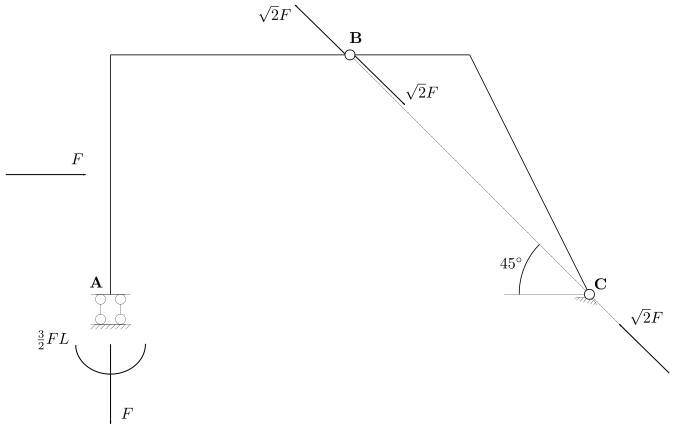
\includegraphics[width=\textwidth]{Immagini/Parte_8/Esercizio8_2/Esercizio8_2_3.pdf}
\caption{}
\label{Esercizio8-2-3}
\end{figure}
%--------------------------------------------------------------------------------------------------------------------------------------------------------------
Il quadro completo delle reazioni è riportato in figura~\ref{Esercizio8-2-3}.
%--------------------------------------------------------------------------------------------------------------------------------------------------------------
\clearpage
\paragraph{Esercizio 8.3}
Si chiede di
\begin{itemize}
\item di dimostrare che la la struttura rappresentata in figura~\ref{Esercizio8-3-1} è $1$ \textsc{volta labile}; 
\item di stabilire quale relazione deve sussistere tra $F_1$ ed $F_2$ affinché la struttura sia in equilibrio;
\item di determinare le reazioni vincolari assumendo valori compatibili per $F_1$ ed $F_2$.
\end{itemize}
%--------------------------------------------------------------------------------------------------------------------------------------------------------------
%--------------------------------------------------------------------------------------------------------------------------------------------------------------
\renewcommand{\thefigure}{8.3~-~1}
\begin{figure}[ht]
\centering
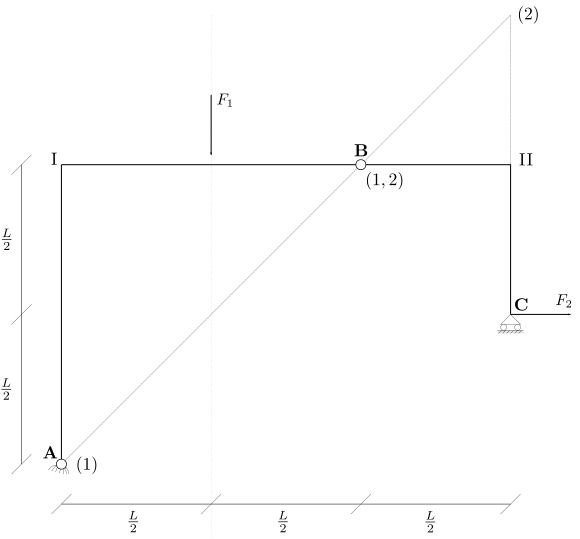
\includegraphics[width=\textwidth]{Immagini/Parte_8/Esercizio8_3/Esercizio8_3_1.pdf}
\caption{}
\label{Esercizio8-3-1}
\end{figure}
%--------------------------------------------------------------------------------------------------------------------------------------------------------------
\noindent \subparagraph{Quesito 1:}
%----------------------------------------------------------------------------------------
\begin{align*}
m &= 2\times 3 = 6 \\
n &= 2\mathbf{A}+2\mathbf{B}+1\mathbf{C} = 5 
\end{align*}
%----------------------------------------------------------------------------------------
per cui
%----------------------------------------------------------------------------------------
\begin{equation*}
m-n = l-i = 1
\end{equation*}
%----------------------------------------------------------------------------------------
Essendo i centri assoluti $(1)$ e $(2)$ ed il centro relativo $(1,2)$ univocamente determinati ed allineati, la struttura è $1$ \textsc{volta labile}. Dunque
%----------------------------------------------------------------------------------------
\begin{align*}
l &= 1 \\
i &= 0
\end{align*}
%----------------------------------------------------------------------------------------
da cui deduciamo che la struttura data è $1$ \textsc{volta labile determinata}.
%----------------------------------------------------------------------------------------
\noindent \subparagraph{Quesito 2:}
%----------------------------------------------------------------------------------------
%--------------------------------------------------------------------------------------------------------------------------------------------------------------
\renewcommand{\thefigure}{8.3~-~2}
\begin{figure}[ht]
\centering
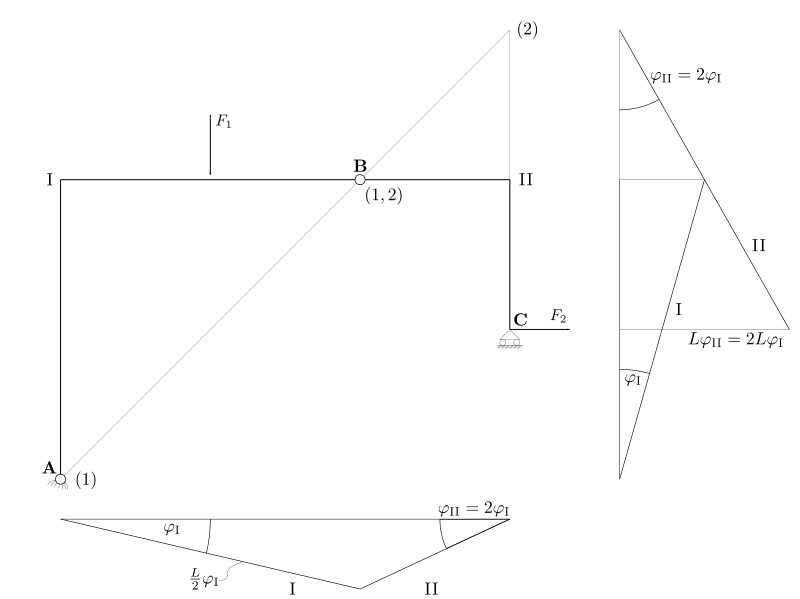
\includegraphics[width=\textwidth]{Immagini/Parte_8/Esercizio8_3/Esercizio8_3_2.pdf}
\caption{}
\label{Esercizio8-3-2}
\end{figure}
%--------------------------------------------------------------------------------------------------------------------------------------------------------------
Troveremo la condizione di compatibilità applicando il \textsc{Principio dei Lavori Virtuali} dei sistemi olonomi. Successivamente vedremo come la stessa relazione scaturisce dalle equazioni di equilibrio. Cominciamo a disegnare un diagramma di spostamenti virtuali, riportato in figura~\ref{Esercizio8-3-2}, al fine di poter esplicitare il lavoro virtuale. Dal disegno si deduce la seguente equazione 
%----------------------------------------------------------------------------------------
\begin{equation*}
\textup{\textsc{Lavoro virtuale}} = L_{v} = F_{1}\frac{L}{2}\varphi_{1} + F_{2}2L\varphi_{1} = \frac{1}{2}(F_{1}+4F_{2})L\varphi_{1}
\end{equation*}
%----------------------------------------------------------------------------------------
Quindi 
%----------------------------------------------------------------------------------------
\begin{equation*}
\boxed{\textup{\textsc{Equilibrio}}} \,\,\iff\,\, L_v = 0, \,\,\forall\varphi_{1} \,\,\iff\,\, F_{1}+4F_{2}=0 \,\,\iff\,\, F_{1} = -4F_{2}
\end{equation*}
%----------------------------------------------------------------------------------------
Il segno negativo implica che una delle due forze deve avere verso opposto a quello disegnato. 
%----------------------------------------------------------------------------------------
\noindent \subparagraph{Quesito 3:}
%--------------------------------------------------------------------------------------------------------------------------------------------------------------
\renewcommand{\thefigure}{8.3~-~3}
\begin{figure}[ht]
\centering
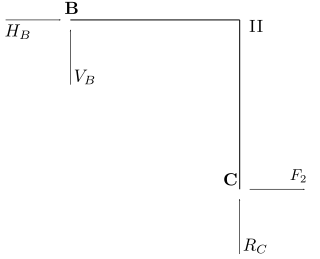
\includegraphics[width=0.55\textwidth]{Immagini/Parte_8/Esercizio8_3/Esercizio8_3_3.pdf}
\caption{}
\label{Esercizio8-3-3}
\end{figure}
%--------------------------------------------------------------------------------------------------------------------------------------------------------------
%----------------------------------------------------------------------------------------
Cominciamo ad imporre l'equilibrio del \textsc{II Tronco}, che è isostatico. Osservando la figura~\ref{Esercizio8-3-3} si ha
%----------------------------------------------------------------------------------------
\begin{align*}
H_B + F_2 &= 0 \quad [\rightarrow] \\
V_B + R_C &= 0 \quad [\uparrow] \\ 
F_{2}\frac{L}{2} + R_{C}\frac{L}{2} &= 0 \quad [\mathbf{B}\circlearrowleft] 
\end{align*}
%----------------------------------------------------------------------------------------
e considerando $F_2$ come \textsc{termine noto}
%----------------------------------------------------------------------------------------
\begin{align*}
H_B &= -F_2  \\
V_B &=  F_2  \\ 
R_C &= -F_2 
\end{align*}
%----------------------------------------------------------------------------------------
%--------------------------------------------------------------------------------------------------------------------------------------------------------------
\renewcommand{\thefigure}{8.3~-~3}
\begin{figure}[ht]
\centering
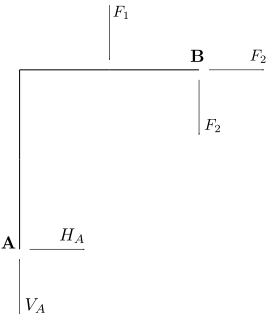
\includegraphics[width=0.55\textwidth]{Immagini/Parte_8/Esercizio8_3/Esercizio8_3_4.pdf}
\caption{}
\label{Esercizio8-3-4}
\end{figure}
%--------------------------------------------------------------------------------------------------------------------------------------------------------------
Ora si passa al \textsc{I Tronco} che, a questo punto, presenta solo due incognite. Osservando la figura~\ref{Esercizio8-3-4}, è possibile scrivere le seguenti
%----------------------------------------------------------------------------------------
\begin{align*}
H_A + F_2 &= 0 \quad [\rightarrow] \\
V_A - F_2 - F_1 &= 0 \quad [\uparrow] \\ 
-F_{1}\frac{L}{2} -F_{2}L - F_{2}L &= 0 \quad [\mathbf{A}\circlearrowleft] 
\end{align*}
%----------------------------------------------------------------------------------------
e dunque
%----------------------------------------------------------------------------------------
\begin{align*}
H_A &= -F_2  \\
V_A &=  F_2+F_1  \\ 
F_2 &= -\frac{1}{4}F_1 
\end{align*}
%----------------------------------------------------------------------------------------
Appare evidente che la terza equazione conduce alla stessa condizione di compatibilità trovata con il Principio dei Lavori Virtuali. Calcoleremo ora le reazioni vincolari assumendo quanto segue
%----------------------------------------------------------------------------------------
\begin{align*}
F_1 &= 4F  \\
F_2 &= -F
\end{align*}
%----------------------------------------------------------------------------------------
e rispettando, così, la condizione di compatibilità, possiamo sfruttare i risultati precedentemente trovati sostituendo in essi $F_1$ con $4F$ ed $F_2$ con $-F$, ottenendo così quanto segue
%----------------------------------------------------------------------------------------
\begin{align*}
H_B &= -F_2 = F \quad [\rightarrow]  \\
R_C &= -F_2 = F \quad [\uparrow] \\
V_B &= F_2 = -F \quad [\downarrow] \\
H_A &= -F_2 = F \quad [\rightarrow] \\ 
V_A &= F_1 + F_2 = 3F \quad [\uparrow] 
\end{align*}
%----------------------------------------------------------------------------------------
%--------------------------------------------------------------------------------------------------------------------------------------------------------------
\renewcommand{\thefigure}{8.3~-~5}
\begin{figure}[ht]
\centering
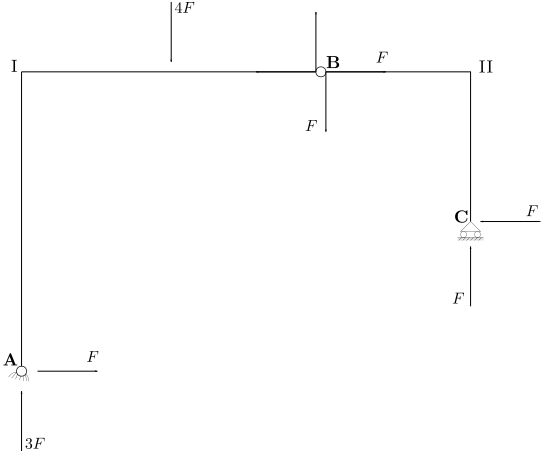
\includegraphics[width=\textwidth]{Immagini/Parte_8/Esercizio8_3/Esercizio8_3_5.pdf}
\caption{}
\label{Esercizio8-3-5}
\end{figure}
%--------------------------------------------------------------------------------------------------------------------------------------------------------------
Il quadro completo delle reazioni viene riportato in figura~\ref{Esercizio8-3-5}.
%----------------------------------------------------------------------------------------